\documentclass[conference,a4paper]{IEEEtran}
\IEEEoverridecommandlockouts

\usepackage[indonesian]{babel}
\usepackage[utf8]{inputenc}
\usepackage[T1]{fontenc}
\usepackage{cite}
\usepackage{amsmath,amssymb}
\usepackage{graphicx}
\usepackage{booktabs}
\usepackage{siunitx}
\usepackage{xcolor}
\usepackage[hidelinks]{hyperref}
\graphicspath{{gambar/}}

% Penanda petunjuk (hapus pemakaiannya di versi akhir)
\newcommand{\petunjuk}[1]{\textcolor{gray}{[#1]}}

\begin{document}

\title{Studi Ablasi RNN, LSTM, dan GRU dibandingkan ANN untuk Prediksi Trafik Seluler Kota Milan}

% Satu blok per anggota (maks. 3). Hapus blok yang tidak dipakai.
\author{
\IEEEauthorblockN{Rossa Amelia Putri}
\IEEEauthorblockA{NIM 124400032\\
Teknik Telekomunikasi, ITERA\\
rossa.124400032@student.itera.ac.id}
\and
\IEEEauthorblockN{Eliada Marcela Bangun}
\IEEEauthorblockA{NIM 124400044\\
Teknik Telekomunikasi, ITERA\\
eliada.124400044@student.itera.ac.id}
\and
\IEEEauthorblockN{Tino Sumandi Siregar}
\IEEEauthorblockA{NIM 124400036\
Teknik Telekomunikasi, ITERA\\
tino.124400036@student.itera.ac.id}
}

\maketitle

\begin{abstract}
Penelitian ini membahas prediksi trafik internet per jam menggunakan dataset Telecom Italia dengan fokus pada lokasi Duomo di Milan. Penelitian bertujuan membandingkan kinerja Artificial Neural Network (ANN), Recurrent Neural Network (RNN), Long Short-Term Memory (LSTM), dan Gated Recurrent Unit (GRU), serta menganalisis pengaruh konfigurasi hiperparameter terhadap akurasi prediksi. Studi ablasi dilakukan dengan menguji lima faktor, yaitu panjang jendela, ukuran hidden, jumlah lapisan, learning rate, dan kelompok fitur. Setiap konfigurasi dijalankan menggunakan tiga random seed dan dievaluasi berdasarkan Mean Absolute Error (MAE). Hasil eksperimen menunjukkan bahwa konfigurasi terbaik GRU memperoleh test MAE sebesar 228,77 ± 6,12, lebih rendah dibandingkan model ANN, RNN, dan LSTM pada konfigurasi terbaik masing-masing. Konfigurasi tersebut menggunakan panjang jendela 48 jam, hidden size 128, dan dua lapisan. Pengujian generalisasi pada Universita Bocconi menghasilkan test MAE sebesar 511,16 ± 41,71 untuk GRU, menunjukkan adanya penurunan kinerja ketika model diterapkan pada lokasi berbeda. Hasil ini menunjukkan bahwa GRU memberikan kinerja prediksi terbaik pada lokasi Duomo, tetapi karakteristik trafik lokasi turut memengaruhi kemampuan generalisasi model.
\petunjuk{150--200 kata. Tuliskan: masalah (prediksi trafik internet per jam), data (Telecom Italia, kotak Duomo dan lokasi kelompok), apa yang diuji (ablasi faktor apa saja, 3 seed), temuan utama dengan angka (misalnya ``GRU terbaik dengan test MAE $x \pm y$, turun $z$\,\% dari acuan''), dan satu kalimat kesimpulan.}
\end{abstract}

\begin{IEEEkeywords}
prediksi trafik seluler, RNN, LSTM, GRU, studi ablasi
\end{IEEEkeywords}

% ---------------------------------------------------------------------
\section{Pendahuluan}
Prediksi trafik internet pada setiap sel atau lokasi jaringan diperlukan oleh operator telekomunikasi untuk memperkirakan kebutuhan kapasitas, mengoptimalkan penggunaan sumber daya jaringan, serta menjaga kualitas layanan. Hal ini penting karena pola penggunaan trafik dapat berbeda pada setiap lokasi dan waktu. Dengan memprediksi trafik berdasarkan data historis, operator dapat mengantisipasi perubahan kebutuhan jaringan dan melakukan pengelolaan kapasitas secara lebih tepat.

Penelitian ini membandingkan Artificial Neural Network (ANN) dengan tiga model sekuensial, yaitu Recurrent Neural Network (RNN), Long Short-Term Memory (LSTM), dan Gated Recurrent Unit (GRU). ANN digunakan sebagai pembanding, sedangkan model sekuensial digunakan untuk mempelajari hubungan temporal dari urutan data trafik. Perbandingan ini bertujuan mengetahui apakah kemampuan model dalam memanfaatkan informasi urutan waktu dapat menghasilkan prediksi yang lebih baik dibandingkan ANN. Selain itu, dilakukan studi ablasi, yaitu pengujian dengan mengubah faktor konfigurasi model untuk mengetahui pengaruh setiap faktor terhadap kinerja prediksi. Studi ini penting agar pemilihan konfigurasi model didasarkan pada hasil evaluasi, bukan hanya asumsi.

Kontribusi penelitian ini adalah:
1. Membandingkan kinerja ANN, RNN, LSTM, dan GRU dalam memprediksi trafik internet per jam pada lokasi Duomo menggunakan dataset Telecom Italia.
2. Menganalisis pengaruh panjang jendela input, ukuran hidden, jumlah lapisan, learning rate, dan kelompok fitur melalui studi ablasi.
3. Mengevaluasi konfigurasi terbaik dan menguji kemampuan generalisasi model pada lokasi lain di Milan

% ---------------------------------------------------------------------
\section{Data dan Metode}

\subsection{Dataset}
Penelitian ini menggunakan dataset Telecom Italia Big Data Challenge \cite{barlacchi2015milan} dengan versi data per jam yang mengacu pada \cite{zhang2021fedda}. Dataset ini berisi aktivitas penggunaan jaringan seluler di wilayah Milan, Italia. Data memiliki resolusi waktu satu jam dan terdiri dari tiga fitur utama, yaitu penggunaan internet (net), panggilan telepon (call), dan pesan singkat (sms).
Pada penelitian ini, data utama yang digunakan berasal dari lokasi Duomo dengan nomor kotak 5060. Data tersebut digunakan untuk melakukan eksperimen dan membandingkan kinerja empat model, yaitu ANN, RNN, LSTM, dan GRU.
Selain lokasi Duomo, penelitian ini juga menggunakan data dari lokasi kelompok untuk menguji kemampuan generalisasi model. Berdasarkan kode lokasi kelompok, lokasi yang digunakan adalah kode 2, yaitu Universita Bocconi dengan nomor kotak 4460.
Peta lokasi penelitian ditampilkan pada Gambar~\ref{fig:peta}. Lingkaran toska menunjukkan lokasi Duomo, sedangkan lingkaran kuning menunjukkan lokasi tugas kelompok.

\begin{figure}[t]
  \centering
  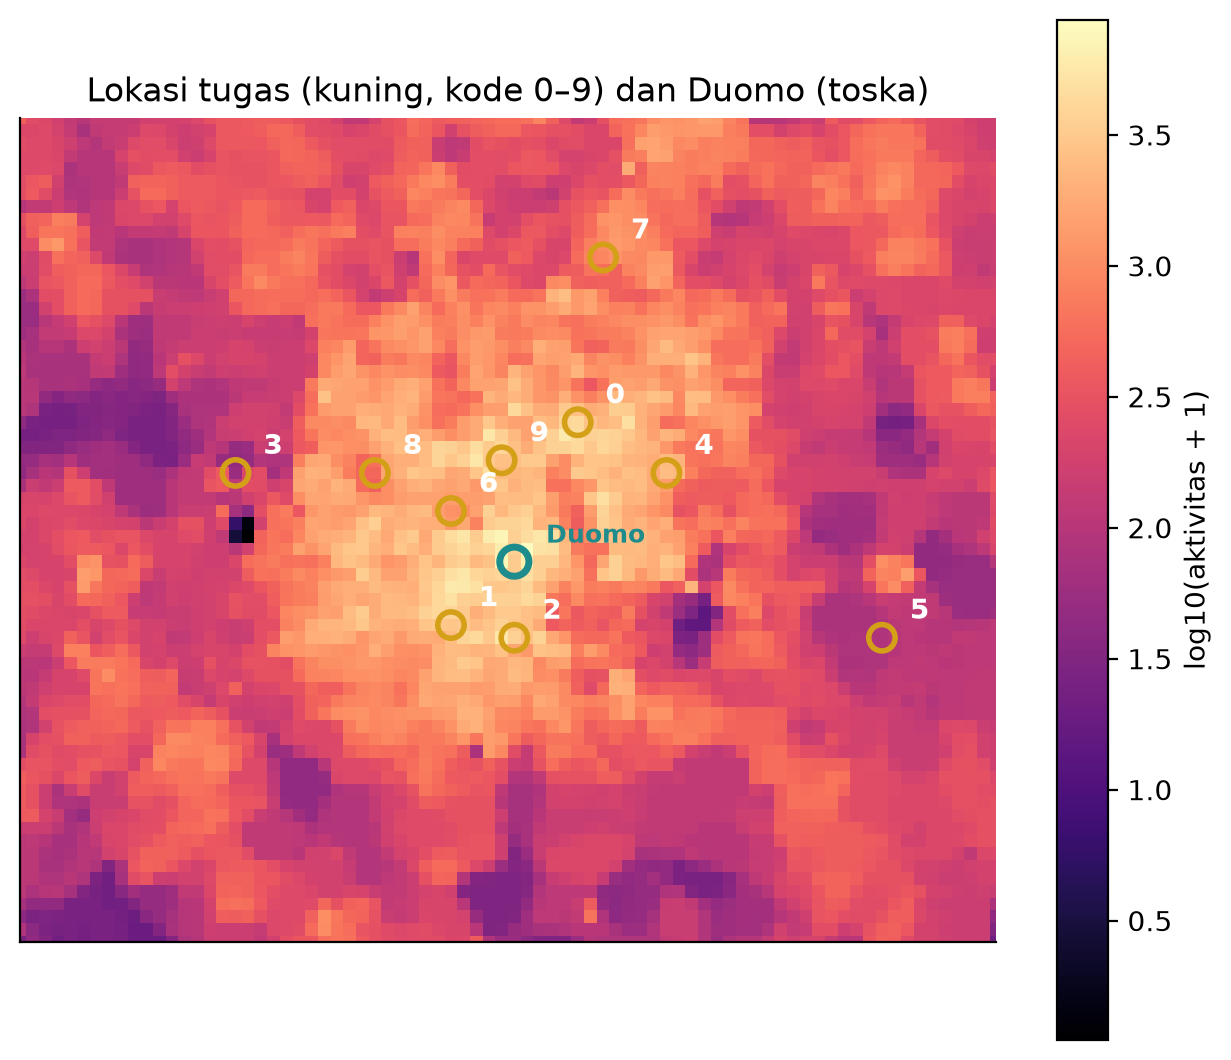
\includegraphics[width=0.85\linewidth]{peta_lokasi_tugas.png}
  \caption{Rata-rata aktivitas internet per kotak di Milan. Lingkaran kuning: lokasi tugas (kode 0--9); lingkaran toska: Duomo.}
  \label{fig:peta}
\end{figure}

\subsection{Pembagian Data dan Praproses}
Pembagian data dilakukan berdasarkan urutan waktu agar proses pelatihan dan evaluasi model mencerminkan kondisi prediksi pada data yang belum pernah dilihat sebelumnya. Data dibagi menjadi empat bagian, yaitu data pelatihan (\textit{training}), validasi (\textit{validation}), pengujian (\textit{testing}), dan periode Natal.

Data pelatihan menggunakan periode 11 November hingga 8 Desember 2013. Selanjutnya, data validasi menggunakan periode 9--15 Desember 2013, sedangkan data pengujian menggunakan periode 16--22 Desember 2013. Periode 23--29 Desember 2013 digunakan sebagai data Natal untuk mengamati kinerja model pada periode dengan pola aktivitas yang berbeda. Data 4--10 November 2013 digunakan sebagai konteks awal untuk membentuk urutan data.

Sebelum digunakan oleh model, data terlebih dahulu melalui proses standarisasi. Standarisasi dilakukan menggunakan nilai rata-rata (\textit{mean}) dan standar deviasi (\textit{standard deviation}) yang dihitung dari data sebelum minggu validasi, yaitu data hingga 8 Desember 2013. Statistik tersebut kemudian digunakan untuk mentransformasikan seluruh bagian data, termasuk validasi, pengujian, dan periode Natal. Cara ini bertujuan agar informasi dari data validasi dan pengujian tidak digunakan dalam proses perhitungan parameter standarisasi.

Setelah standarisasi, data diubah menjadi pasangan input dan target menggunakan metode \textit{windowing}. Metode ini membentuk urutan data berdasarkan sejumlah jam sebelumnya (\textit{window}) untuk memprediksi nilai pada waktu berikutnya (\textit{horizon}). Pada konfigurasi acuan, panjang \textit{window} adalah 24 jam dan \textit{horizon} adalah 1 jam. Dengan demikian, model menggunakan data 24 jam sebelumnya untuk memprediksi aktivitas pada satu jam berikutnya.

Pembagian data deret waktu tidak boleh dilakukan secara acak karena urutan waktu merupakan bagian penting dari informasi data. Jika data diacak, informasi dari waktu yang lebih baru dapat masuk ke data pelatihan, sementara data dari waktu yang lebih lama masuk ke data pengujian. Hal tersebut dapat menyebabkan kebocoran informasi (\textit{data leakage}) dan membuat hasil evaluasi tidak menggambarkan kemampuan model dalam memprediksi masa depan. Oleh karena itu, pembagian dilakukan secara kronologis, yaitu data pelatihan berasal dari periode paling awal, diikuti data validasi, pengujian, dan periode Natal.

\subsection{Model dan Konfigurasi Acuan}
Penelitian ini membandingkan empat jenis model jaringan saraf, yaitu Artificial Neural Network (ANN), Recurrent Neural Network (RNN), Long Short-Term Memory (LSTM), dan Gated Recurrent Unit (GRU).

ANN merupakan jaringan saraf yang memproses masukan melalui beberapa lapisan neuron untuk mempelajari hubungan antara fitur masukan dan nilai yang diprediksi. Pada penelitian ini, data dari beberapa jam sebelumnya diubah menjadi satu vektor masukan sebelum diproses oleh ANN.

RNN merupakan jaringan saraf yang dirancang untuk memproses data berurutan. Model ini memiliki koneksi berulang sehingga informasi dari langkah waktu sebelumnya dapat digunakan untuk memproses langkah waktu berikutnya. Dengan kemampuan tersebut, RNN dapat mempelajari pola temporal pada data aktivitas jaringan seluler.

LSTM merupakan pengembangan RNN yang menggunakan mekanisme gerbang (\textit{gates}) untuk mengatur informasi yang disimpan, dilupakan, dan diteruskan. Mekanisme ini membantu model mempelajari ketergantungan jangka panjang dan mengurangi masalah hilangnya informasi pada urutan yang panjang.

GRU juga merupakan pengembangan RNN yang menggunakan mekanisme gerbang untuk mengatur aliran informasi. Dibandingkan LSTM, GRU memiliki struktur yang lebih sederhana karena menggunakan lebih sedikit gerbang, sehingga berpotensi membutuhkan komputasi yang lebih ringan.

Keempat model dilatih menggunakan konfigurasi acuan yang ditunjukkan pada Tabel~\ref{tab:acuan}. Konfigurasi ini digunakan sebagai dasar perbandingan sebelum dilakukan eksperimen perubahan hiperparameter.

\begin{table}[t]
  \centering
  \caption{Konfigurasi acuan}
  \label{tab:acuan}
  \begin{tabular}{@{}ll@{}}
    \toprule
    Hyperparameter & Nilai acuan \\
    \midrule
    Panjang jendela $W$ & 24 jam \\
    Horizon & 1 jam \\
    Ukuran hidden & ANN 32, RNN 68, LSTM 33, GRU 38 \\
    Jumlah lapisan & ANN 2, rekuren 1 \\
    Fitur & net, call, sms, jam, hari (7) \\
    Optimizer, \textit{learning rate} & Adam, $10^{-3}$ \\
    \textit{Batch size} & 64 \\
    \textit{Early stopping} & \textit{patience} 30, maks.\ 300 epoch \\
    \bottomrule
  \end{tabular}
\end{table}

\subsection{Protokol Ablasi dan Evaluasi}
Eksperimen dilakukan pada data trafik jaringan seluler di lokasi Duomo, Milan, menggunakan pembagian waktu yang sama dengan Sesi 2. Data 4--10 November 2013 digunakan sebagai konteks jendela, 11 November--8 Desember sebagai data pelatihan, 9--15 Desember sebagai validasi, 16--22 Desember sebagai pengujian, dan 23--29 Desember sebagai periode Natal. Standardisasi fitur menggunakan rata-rata dan standar deviasi yang dihitung dari data sebelum 9 Desember, kemudian diterapkan pada seluruh periode untuk menghindari penggunaan informasi masa depan. Model menggunakan data selama $W$ jam sebelumnya untuk memprediksi trafik pada horizon $H=1$ jam.

Ablasi menggunakan pendekatan \textit{one-factor-at-a-time}, yaitu mengubah satu faktor dan mempertahankan parameter lainnya sesuai konfigurasi acuan. Lima faktor wajib yang diuji meliputi: (A1) panjang jendela input $W \in \{6,12,24,48,168\}$; (A2) ukuran \textit{hidden} $\in \{16,32,64,128\}$; (A3) jumlah lapisan $\in \{1,2,3\}$; (A4) \textit{learning rate} $\in \{0.0001,0.001,0.01\}$; dan (A5) kelompok fitur, yaitu \textit{net}, \textit{net+call+sms}, \textit{net+waktu}, serta \textit{semua}. Pengujian fitur bertujuan mengetahui kontribusi informasi penggunaan layanan dan waktu terhadap prediksi. Selain itu, dipilih dua faktor tambahan, yaitu (B2) \textit{dropout} dengan nilai $\{0,0.2,0.5\}$ untuk menguji pengaruh regularisasi terhadap \textit{overfitting}, serta (B4) fungsi \textit{loss} MSE, MAE, dan Huber untuk membandingkan pengaruh fungsi kesalahan terhadap hasil pelatihan.

Konfigurasi acuan menggunakan $W=24$, $H=1$, \textit{batch size} 64, \textit{learning rate} 0.001, optimizer Adam, \textit{dropout} 0, \textit{loss} MSE, \textit{early stopping patience} 30, dan maksimum 300 epoch. Ukuran \textit{hidden} masing-masing model adalah 32 untuk ANN, 68 untuk RNN, 33 untuk LSTM, dan 38 untuk GRU. Jumlah lapisan acuan adalah dua untuk ANN dan satu untuk model rekuren. Model yang dibandingkan meliputi ANN, RNN, LSTM, dan GRU. Pada ANN, jendela input diratakan sebelum masuk ke lapisan tersembunyi, sedangkan model rekuren memproses urutan waktu dan menggunakan \textit{hidden state} pada jam terakhir untuk menghasilkan prediksi.

Setiap konfigurasi dijalankan menggunakan tiga \textit{random seed}, yaitu 0, 1, dan 2. Hasil dilaporkan dalam bentuk rata-rata $\pm$ simpangan baku. Evaluasi menggunakan MAE, RMSE, dan MAPE yang dihitung pada skala asli setelah proses \textit{inverse standardization}. Pemilihan konfigurasi terbaik untuk setiap model didasarkan pada MAE validasi terendah. Data test dan Natal hanya digunakan untuk pelaporan performa akhir, bukan untuk memilih konfigurasi. Selanjutnya, konfigurasi terbaik diuji pada lokasi kelompok untuk mengevaluasi kemampuan generalisasi model di lokasi berbeda. Hasil model juga dibandingkan dengan baseline naif, yaitu prediksi berdasarkan nilai terakhir, nilai pada 24 jam sebelumnya, dan nilai pada 168 jam sebelumnya.

Eksperimen dijalankan menggunakan PyTorch pada CPU. Waktu pelatihan setiap eksperimen dicatat untuk mengevaluasi kebutuhan komputasi. Berdasarkan akumulasi durasi eksperimen yang tercatat, waktu pelatihan mencapai sekitar 110,6 menit; angka ini mengikuti catatan durasi yang tersedia.
```
% ---------------------------------------------------------------------
\section{Hasil}

\subsection{Baseline Naif dan Acuan}
Baseline naif digunakan sebagai pembanding untuk mengetahui apakah model mampu menghasilkan prediksi yang lebih baik daripada metode sederhana tanpa pelatihan. Tiga metode yang digunakan adalah nilai trafik terakhir, nilai pada 24 jam sebelumnya (kemarin), dan nilai pada 168 jam sebelumnya (minggu lalu). Tabel~\ref{tab:baseline} menunjukkan hasil MAE pada lokasi Duomo untuk horizon prediksi satu jam.

\begin{table}[ht]
\centering
\caption{MAE baseline naif pada lokasi Duomo (horizon 1 jam).}
\label{tab:baseline}
\small
\begin{tabular}{lrrr}
\hline
\textbf{Metode} & \textbf{Validasi} & \textbf{Test} & \textbf{Natal} \\
\hline
Nilai terakhir & 662.6 & 600.9 & 431.2 \\
Nilai kemarin & 595.3 & 552.2 & 921.5 \\
Nilai minggu lalu & 492.8 & 467.6 & 1426.2 \\
\hline
\end{tabular}
\end{table}

Hasil menunjukkan bahwa baseline nilai minggu lalu memperoleh MAE terendah pada validasi dan test, masing-masing sebesar 492.8 dan 467.6. Sementara itu, pada periode Natal, baseline nilai terakhir memberikan hasil terbaik dengan MAE 431.2. Perbedaan ini menunjukkan bahwa pola trafik pada periode Natal tidak sepenuhnya mengikuti pola mingguan sebelumnya.

Selanjutnya, konfigurasi acuan ANN, RNN, LSTM, dan GRU dievaluasi menggunakan tiga \textit{random seed}. Tabel~\ref{tab:acuan} menyajikan rata-rata dan simpangan baku metrik evaluasi pada validasi, test, dan Natal.

\begin{table}[ht]
\centering
\caption{Hasil konfigurasi acuan pada lokasi Duomo (rata-rata $\pm$ simpangan baku).}
\label{tab:acuan}
\scriptsize
\begin{tabular}{llrrr}
\hline
\textbf{Model} & \textbf{Split} & \textbf{MAE} & \textbf{RMSE} & \textbf{MAPE (\%)} \\
\hline
ANN & Validasi & $248.9 \pm 8.9$ & $372.4 \pm 12.3$ & $7.8 \pm 0.6$ \\
    & Test     & $309.9 \pm 5.9$ & $445.6 \pm 19.5$ & $11.3 \pm 0.8$ \\
    & Natal    & $680.1 \pm 52.0$ & $969.6 \pm 41.6$ & $50.0 \pm 4.9$ \\
\hline
RNN & Validasi & $206.1 \pm 7.4$ & $309.3 \pm 17.7$ & $6.6 \pm 0.1$ \\
    & Test     & $229.6 \pm 5.1$ & $338.4 \pm 18.1$ & $8.5 \pm 0.3$ \\
    & Natal    & $421.2 \pm 2.4$ & $561.7 \pm 17.3$ & $30.2 \pm 0.6$ \\
\hline
LSTM & Validasi & $230.5 \pm 12.2$ & $331.4 \pm 13.5$ & $6.5 \pm 0.5$ \\
     & Test     & $273.6 \pm 25.4$ & $417.0 \pm 37.4$ & $9.1 \pm 1.0$ \\
     & Natal    & $586.0 \pm 56.8$ & $777.1 \pm 92.4$ & $43.4 \pm 5.9$ \\
\hline
GRU & Validasi & $207.5 \pm 3.8$ & $303.3 \pm 12.6$ & $6.1 \pm 0.1$ \\
    & Test     & $237.2 \pm 9.3$ & $360.2 \pm 14.0$ & $8.0 \pm 0.7$ \\
    & Natal    & $468.2 \pm 21.8$ & $627.9 \pm 16.2$ & $33.7 \pm 2.6$ \\
\hline
\end{tabular}
\end{table}

Berdasarkan hasil konfigurasi acuan, RNN memperoleh MAE validasi dan test terendah, masing-masing 206.1 dan 229.6. GRU menghasilkan MAPE terendah pada kedua split tersebut, yaitu 6.1\% pada validasi dan 8.0\% pada test. Pada periode Natal, RNN juga memberikan MAE terendah sebesar 421.2. Secara umum, keempat model memiliki error lebih tinggi pada periode Natal dibandingkan periode test. Hal ini mengindikasikan adanya perubahan pola trafik pada periode tersebut. Seluruh model juga memiliki MAE lebih rendah dibandingkan ketiga baseline naif pada validasi dan test, sehingga model pembelajaran mampu menangkap pola trafik lebih baik daripada metode sederhana.

\subsection{Ablasi Wajib}
Ablasi wajib dilakukan dengan mengubah satu faktor pada satu waktu, yaitu panjang jendela ($W$), ukuran hidden layer, jumlah layer, learning rate, dan kombinasi fitur masukan. Hasil pengujian dievaluasi menggunakan test MAE dan disajikan sebagai rata-rata $\pm$ simpangan baku dari tiga seed. Ringkasan seluruh hasil ditampilkan pada Tabel~\ref{tab:ablasi-gabungan}.

\begin{table}[ht]
\centering
\caption{Ringkasan hasil ablasi wajib berdasarkan test MAE (rata-rata $\pm$ simpangan baku dari 3 seed).}
\label{tab:ablasi-gabungan}
\scriptsize
\begin{tabular}{@{}llcccc@{}}
\toprule
Faktor & Pengaturan & ANN & RNN & LSTM & GRU \\
\midrule
\multicolumn{6}{l}{\textbf{A1 -- Panjang jendela ($W$)}}\\
& 6 & $269.4 \pm 16.8$ & $228.6 \pm 5.4$ & $276.3 \pm 14.7$ & $249.8 \pm 1.4$\\
& 12 & $308.8 \pm 11.6$ & $233.2 \pm 11.2$ & $302.7 \pm 17.4$ & $246.1 \pm 13.5$\\
& 24 & $309.9 \pm 5.9$ & $229.6 \pm 5.1$ & $273.6 \pm 25.4$ & $237.2 \pm 9.3$\\
& 48 & $333.1 \pm 20.3$ & $\mathbf{224.5 \pm 11.7}$ & $304.4 \pm 27.1$ & $\mathbf{237.1 \pm 10.6}$\\
& 168 & $402.0 \pm 12.5$ & $233.5 \pm 4.8$ & $292.8 \pm 20.0$ & $237.2 \pm 10.6$\\
\midrule
\multicolumn{6}{l}{\textbf{A2 -- Ukuran hidden layer}}\\
& 16 & $312.1 \pm 19.3$ & $253.3 \pm 9.3$ & $295.3 \pm 13.1$ & $246.9 \pm 10.4$\\
& 32 & $309.9 \pm 5.9$ & $245.2 \pm 3.7$ & $290.8 \pm 20.9$ & $232.7 \pm 5.1$\\
& 64 & $316.2 \pm 24.2$ & $240.9 \pm 15.0$ & $269.2 \pm 12.7$ & $225.0 \pm 12.7$\\
& 128 & $\mathbf{296.8 \pm 32.2}$ & $\mathbf{234.6 \pm 18.6}$ & $\mathbf{245.6 \pm 6.7}$ & $\mathbf{220.3 \pm 10.6}$\\
\midrule
\multicolumn{6}{l}{\textbf{A3 -- Jumlah layer}}\\
& 1 & $311.8 \pm 11.0$ & $229.6 \pm 5.1$ & $\mathbf{273.6 \pm 25.4}$ & $\mathbf{237.2 \pm 9.3}$\\
& 2 & $309.9 \pm 5.9$ & $\mathbf{228.4 \pm 8.2}$ & $308.9 \pm 20.6$ & $239.2 \pm 6.4$\\
& 3 & $\mathbf{299.8 \pm 25.1}$ & $245.5 \pm 19.1$ & $412.6 \pm 54.2$ & $264.2 \pm 11.4$\\
\midrule
\multicolumn{6}{l}{\textbf{A4 -- Learning rate}}\\
& 0.0001 & $339.7 \pm 22.5$ & $287.9 \pm 7.3$ & $373.5 \pm 14.3$ & $356.3 \pm 7.9$\\
& 0.001 & $\mathbf{309.9 \pm 5.9}$ & $\mathbf{229.6 \pm 5.1}$ & $273.6 \pm 25.4$ & $237.2 \pm 9.3$\\
& 0.01 & $309.4 \pm 53.2$ & $245.8 \pm 12.3$ & $\mathbf{225.8 \pm 4.2}$ & $\mathbf{215.7 \pm 10.9}$\\
\midrule
\multicolumn{6}{l}{\textbf{A5 -- Kombinasi fitur}}\\
& \texttt{net} & $\mathbf{271.8 \pm 13.8}$ & $254.1 \pm 1.7$ & $284.2 \pm 19.3$ & $270.5 \pm 10.9$\\
& \texttt{net+call+sms} & $315.9 \pm 12.2$ & $\mathbf{227.6 \pm 2.2}$ & $\mathbf{262.7 \pm 10.9}$ & $250.7 \pm 9.3$\\
& \texttt{net+waktu} & $296.4 \pm 9.1$ & $244.9 \pm 22.1$ & $292.6 \pm 25.1$ & $239.7 \pm 25.4$\\
& \texttt{semua} & $309.9 \pm 5.9$ & $229.6 \pm 5.1$ & $273.6 \pm 25.4$ & $\mathbf{237.2 \pm 9.3}$\\
\bottomrule
\end{tabular}
\end{table}

Pada A1, panjang jendela terbaik berbeda antararsitektur. RNN dan GRU memperoleh MAE terendah pada $W=48$, sedangkan ANN dan LSTM terbaik pada $W=6$. Pada A2, ukuran hidden layer 128 menghasilkan MAE terendah untuk seluruh arsitektur. Pada A3, ANN terbaik dengan 3 layer, RNN dengan 2 layer, sedangkan LSTM dan GRU dengan 1 layer. Hasil ini menunjukkan bahwa penambahan jumlah layer tidak selalu meningkatkan performa.

Pada A4, learning rate $0.001$ memberikan hasil terbaik untuk ANN dan RNN, sedangkan $0.01$ terbaik untuk LSTM dan GRU. Pada A5, ANN memperoleh hasil terbaik dengan fitur \texttt{net}, RNN dan LSTM dengan \texttt{net+call+sms}, serta GRU dengan \texttt{semua}. Dengan demikian, konfigurasi fitur terbaik bergantung pada arsitektur yang digunakan. Grafik seluruh faktor ablasi ditampilkan secara gabungan pada Gambar~\ref{fig:ablasi-gabungan}.

\subsection{Ablasi Pilihan}
\noindent\textbf{B2: Pengaruh Dropout.} Hipotesis awal menyatakan bahwa dropout sedang dapat mengurangi overfitting dan meningkatkan generalisasi, sedangkan dropout terlalu besar dapat menurunkan akurasi. Pengujian dilakukan menggunakan dropout 0; 0,2; dan 0,5 pada empat model dengan tiga random seed. Hasil menunjukkan bahwa dropout 0,2 menurunkan Validation MAE GRU dari 207,5 menjadi 203,9 dan Test MAE dari 237,2 menjadi 225,0. Pada LSTM, Test MAE juga menurun dari 273,6 menjadi 264,6, tetapi Validation MAE sedikit meningkat. Sebaliknya, ANN dan RNN mengalami peningkatan kesalahan, sedangkan dropout 0,5 memperburuk hasil validasi seluruh model. Dengan demikian, hipotesis hanya terbukti sebagian karena efektivitas dropout bergantung pada arsitektur dan tingkat regularisasi.

\begin{table}[t]
\centering
\caption{Perbandingan MAE konfigurasi acuan, terbaik, dan baseline naif}
\label{tab:konfigurasi-terbaik}
\resizebox{\columnwidth}{!}{
\begin{tabular}{llccc}
ANN  & Acuan   & 248,9 & 309,9 & 680,1 \\
ANN  & Terbaik & 211,5 & 269,4 & 532,5 \\
RNN  & Acuan   & 206,1 & 229,6 & 421,2 \\
RNN  & Terbaik & 200,1 & 224,5 & 404,5 \\
LSTM & Acuan   & 230,5 & 273,6 & 586,0 \\
LSTM & Terbaik & 207,1 & 245,6 & 491,1 \\
GRU  & Acuan   & 207,5 & 237,2 & 468,2 \\
GRU  & Terbaik & 188,7 & 220,3 & 435,2 \\
\hline
Naif & Kemarin        & 595,3 & 552,2 & 921,5 \\
Naif & Minggu lalu    & 492,8 & 467,6 & 1426,2 \\
Naif & Nilai terakhir & 662,6 & 600,9 & 431,2 \\
\hline
\end{tabular}
}
\end{table}

Berdasarkan Tabel~\ref{tab:konfigurasi-terbaik}, seluruh konfigurasi terbaik menghasilkan MAE lebih rendah dibandingkan konfigurasi acuan. GRU memberikan Validation MAE terendah sebesar 188,7 dan Test MAE terendah sebesar 220,3. Seluruh model terbaik juga mengungguli baseline naif pada minggu pengujian, dengan Test MAE baseline terendah sebesar 467,6. Namun, pada periode Natal, RNN memperoleh hasil terbaik dengan MAE 404,5, lebih rendah daripada baseline naif nilai terakhir sebesar 431,2. GRU menghasilkan Natal MAE 435,2, sedikit lebih tinggi daripada baseline tersebut. Hal ini menunjukkan bahwa pemilihan berdasarkan Validation MAE belum tentu memberikan akurasi terbaik pada periode Natal akibat perubahan karakteristik trafik.


\subsection{Uji Generalisasi}
Uji generalisasi dilakukan pada lokasi Universita Bocconi (kode 2) untuk mengevaluasi kemampuan model ANN, RNN, LSTM, dan GRU pada lokasi berbeda dari Duomo. Setiap model dilatih ulang menggunakan konfigurasi acuan dan konfigurasi terbaik dari hasil ablasi dengan tiga random seed. Perbandingan hasil ditampilkan pada Tabel~\ref{tab:generalisasi}.

\begin{table}[t]
\centering
\caption{Perbandingan MAE di Universita Bocconi}
\label{tab:generalisasi}
\resizebox{\columnwidth}{!}{
\begin{tabular}{llccc}
\hline
\textbf{Model} & \textbf{Konfig.} & \textbf{Val MAE} & \textbf{Test MAE} & \textbf{Natal MAE} \\
\hline
ANN & Acuan & 370,0 & 645,5 & 817,3 \\
ANN & Terbaik & 345,4 & 599,7 & 766,5 \\
RNN & Acuan & 364,5 & 754,2 & 1100,3 \\
RNN & Terbaik & 325,7 & 612,9 & 866,5 \\
LSTM & Acuan & 375,5 & 682,1 & 1240,3 \\
LSTM & Terbaik & 311,6 & 777,4 & 1314,1 \\
GRU & Acuan & 354,7 & 608,5 & 836,9 \\
GRU & Terbaik & 329,1 & 511,2 & 690,1 \\
\hline
\end{tabular}
}
\end{table}

Berdasarkan Tabel~\ref{tab:generalisasi}, konfigurasi terbaik menurunkan Test MAE ANN dari 645,5 menjadi 599,7, RNN dari 754,2 menjadi 612,9, dan GRU dari 608,5 menjadi 511,2. Sebaliknya, Test MAE LSTM meningkat dari 682,1 menjadi 777,4 meskipun Validation MAE menurun. Urutan model pada konfigurasi acuan adalah GRU, ANN, LSTM, dan RNN, sedangkan pada konfigurasi terbaik berubah menjadi GRU, ANN, RNN, dan LSTM. Dengan demikian, GRU tetap menjadi model terbaik, tetapi urutan RNN dan LSTM mengalami perubahan.

Berdasarkan Gambar~\ref{fig:pola-generalisasi}, Duomo memiliki pola trafik harian yang relatif berulang dengan puncak sekitar 6000--9000, sedangkan Universita Bocconi menunjukkan puncak lebih tinggi hingga sekitar 18000 serta penurunan aktivitas yang tajam menjelang akhir Desember. Perbedaan pola trafik tersebut dapat memengaruhi kemampuan generalisasi model. Pada periode Natal, GRU terbaik menghasilkan MAE terendah sebesar 690,1, sedangkan LSTM menghasilkan MAE tertinggi sebesar 1314,1. Hal ini menunjukkan bahwa konfigurasi optimal di Duomo belum tentu memberikan peningkatan kinerja yang konsisten di Universita Bocconi, terutama ketika karakteristik trafik mengalami perubahan.

% ---------------------------------------------------------------------

\section{Pembahasan}
Hasil studi ablasi menunjukkan bahwa pengaruh hiperparameter terhadap akurasi prediksi berbeda pada setiap arsitektur model. Pada eksperimen A1, penambahan panjang jendela tidak selalu meningkatkan akurasi. ANN memperoleh Test MAE sebesar 269,4 pada $W=6$, tetapi meningkat menjadi 402,0 pada $W=168$. Hal ini diduga berkaitan dengan bertambahnya jumlah parameter ANN dari 2465 menjadi 38753 sehingga meningkatkan kompleksitas model dan potensi overfitting pada data latih terbatas. Sebaliknya, RNN, LSTM, dan GRU menggunakan bobot berulang sehingga jumlah parameternya tidak bertambah ketika panjang jendela diperbesar. Namun, informasi historis yang terlalu panjang belum tentu relevan untuk memprediksi trafik satu jam berikutnya.

Pada eksperimen A2 dan A3, peningkatan kapasitas dan kedalaman jaringan juga tidak selalu menghasilkan akurasi lebih baik. GRU memperoleh Validation MAE terendah sebesar 188,7 pada hidden 128, sedangkan LSTM mengalami peningkatan Validation MAE dari 230,5 pada satu lapisan menjadi 338,9 pada tiga lapisan. Kondisi ini kemungkinan berkaitan dengan meningkatnya kompleksitas optimasi ketika jumlah lapisan bertambah. Pada A4, learning rate terlalu kecil, yaitu $10^{-4}$, cenderung menghasilkan kesalahan lebih tinggi karena pembaruan parameter berlangsung lambat. Namun, learning rate yang lebih besar tidak selalu memperburuk hasil karena pengaruhnya bergantung pada arsitektur model. Sementara itu, A5 menunjukkan bahwa fitur waktu membantu model mengenali pola periodik trafik. Pada GRU, Validation MAE menurun dari 264,6 menggunakan fitur net saja menjadi 207,5 ketika seluruh fitur digunakan. Hal ini menunjukkan bahwa informasi masukan yang relevan dapat memberikan manfaat lebih besar daripada sekadar meningkatkan kompleksitas jaringan.

Eksperimen B2 menunjukkan bahwa penggunaan dropout tidak selalu meningkatkan generalisasi. Dropout 0,2 menurunkan Test MAE GRU dari 237,2 menjadi 225,0, tetapi meningkatkan kesalahan pada ANN dan RNN. Dropout 0,5 juga memperburuk kinerja pengujian seluruh model. Hal ini diduga karena regularisasi yang terlalu besar mengurangi informasi yang diperlukan selama pembelajaran. Pada B4, penggunaan loss MAE menurunkan Test MAE RNN dari 229,6 menjadi 207,1, tetapi Validation MAE meningkat dari 206,1 menjadi 217,9. Perbedaan tersebut menunjukkan bahwa fungsi loss yang menghasilkan kinerja pengujian lebih baik belum tentu menghasilkan validasi terbaik. Oleh karena itu, pemilihan konfigurasi tetap didasarkan pada Validation MAE agar data pengujian tidak digunakan dalam proses pemilihan model.

Perbedaan kinerja antararsitektur juga perlu mempertimbangkan variasi hasil antar-random seed. Pada konfigurasi acuan, RNN memperoleh Test MAE sebesar $229,6 \pm 5,1$, sedangkan GRU sebesar $237,2 \pm 9,3$. Selisih rata-rata keduanya relatif kecil jika dibandingkan dengan variasi hasil antar-seed, sehingga belum cukup untuk memastikan bahwa salah satu model selalu lebih unggul. Penggunaan tiga random seed membantu menggambarkan kestabilan pelatihan, tetapi belum cukup untuk memastikan signifikansi statistik perbedaan kinerja.

Uji generalisasi pada Universita Bocconi menunjukkan bahwa konfigurasi terbaik dari Duomo tidak selalu memberikan peningkatan yang konsisten. GRU menghasilkan Test MAE terendah sebesar 511,2, sedangkan LSTM mengalami peningkatan Test MAE dari 682,1 menjadi 777,4 meskipun Validation MAE menurun. Berdasarkan Gambar~\ref{fig:pola-generalisasi}, Duomo memiliki pola aktivitas harian yang relatif berulang, sedangkan Universita Bocconi menunjukkan puncak trafik lebih tinggi dan penurunan aktivitas yang tajam menjelang akhir Desember. Perbedaan karakteristik tersebut diduga menyebabkan perubahan distribusi trafik antara periode pelatihan dan pengujian sehingga pola yang dipelajari model tidak selalu sesuai dengan kondisi berikutnya. Pada periode Natal, GRU tetap memperoleh MAE terendah sebesar 690,1 di antara keempat model.

Keterbatasan penelitian ini meliputi penggunaan data dari satu kota, periode pelatihan yang relatif singkat, satu pembagian data berdasarkan waktu, serta evaluasi pada dua lokasi dengan tiga random seed. Kondisi tersebut membatasi kemampuan penelitian dalam memastikan kestabilan hasil pada periode dan lokasi berbeda. Penelitian selanjutnya dapat menggunakan data lebih panjang, lebih banyak lokasi, serta beberapa pembagian waktu pengujian untuk mengevaluasi kemampuan generalisasi model secara lebih menyeluruh.


\section{Kesimpulan}
Studi ablasi menunjukkan bahwa panjang jendela, ukuran hidden, jumlah lapisan, learning rate, kombinasi fitur, dropout, dan fungsi loss memengaruhi akurasi prediksi trafik seluler, tetapi peningkatan kompleksitas model tidak selalu menghasilkan kinerja lebih baik. Pada lokasi Duomo, GRU dengan hidden 128 memperoleh Validation MAE terendah sebesar 188,7 dan Test MAE sebesar 220,3, lebih baik dibandingkan konfigurasi acuan sebesar 237,2 dan baseline naif terbaik sebesar 467,6. Pada periode Natal di Duomo, RNN menghasilkan MAE terendah sebesar 404,5, lebih baik dibandingkan baseline naif nilai terakhir sebesar 431,2. Uji generalisasi di Universita Bocconi (kode 2) menunjukkan bahwa GRU tetap menghasilkan Test MAE terendah sebesar 511,2 dan Natal MAE sebesar 690,1, sedangkan LSTM mengalami peningkatan Test MAE dari 682,1 menjadi 777,4 setelah penerapan konfigurasi terbaik. Hasil ini menunjukkan bahwa konfigurasi optimal pada satu lokasi belum tentu memberikan peningkatan yang konsisten pada lokasi dan periode berbeda karena adanya perbedaan karakteristik serta pola trafik.

\section*{Kontribusi Anggota}
\begin{tabular}{@{}p{0.35\linewidth}p{0.60\linewidth}@{}}
Rossa Amelia Putri & Pengolahan dataset, pelaksanaan eksperimen A1--A2, analisis hasil, serta penyusunan pendahuluan dan metode penelitian. \\
Eliada Marcela Bangun & Pelaksanaan eksperimen A3--A5, pengujian B2 (dropout), analisis hasil, serta pembuatan tabel dan grafik eksperimen. \\
Tino Sumandi Siregar & Pelaksanaan eksperimen B4 (loss function), pemilihan konfigurasi terbaik, uji generalisasi pada Universita Bocconi, serta penyusunan pembahasan dan kesimpulan. \\
\end{tabular}

\
\section*{Pernyataan Penggunaan AI}
Dalam penyelesaian tugas ini, kelompok menggunakan ChatGPT sebagai alat bantu untuk memahami konsep deep learning, membantu mengidentifikasi dan memperbaiki kesalahan kode Python, menginterpretasikan hasil eksperimen, serta merapikan bahasa dan struktur laporan dalam format LaTeX. Seluruh proses pelatihan model, pengujian, dan pengumpulan data hasil eksperimen dilakukan oleh anggota kelompok menggunakan Jupyter Notebook. Seluruh angka, tabel, dan grafik yang dilaporkan bersumber dari hasil eksperimen kelompok sendiri. Penggunaan AI hanya bersifat pendukung dan tidak menggantikan proses eksperimen maupun evaluasi hasil.

\
\section*{Kode dan Data}
Seluruh kode program, Jupyter Notebook beserta output, hasil eksperimen A1--A5, B2, B4, konfigurasi terbaik, uji generalisasi, grafik, tabel, serta laporan LaTeX tersedia pada repository GitHub kelompok di \url{https://github.com/eliadamarcela/dlw-tugas-ra-124400032}.


\bibliographystyle{IEEEtran}
\bibliography{references}

\end{document}
